\documentclass{article}

\usepackage[spanish]{babel}
\usepackage[numbers,sort&compress]{natbib}
\usepackage[T1]{fontenc}
\usepackage[ansinew]{inputenc}
\usepackage{graphicx}
\usepackage{url}
\usepackage{caption}
\usepackage{subcaption}


\title{Pr\'actica 3: Teor\'ia de colas}
\author{Anahi Llano}
\begin{document}
\maketitle

\section{Introducci\'{o}n.}\label{into}

Se realiza la tercera pr\'actica \cite{elisa} llamada teor\'ia de colas.
 
\section{Metodolog\'{i}a.}\label{met}

Se tomaron en cuenta los c\'odigos mostrados durante clase \citep{elisa1}, para adaptarlos y de esta manera examinar las diferencias en los tiempos de ejecucion  variando el n\'umero de nucleos que como se observa en la imagen  solo se pudo variar de uno y dos nucleos utilizados para llevar a cabo el an\'alisis.

\begin{figure}
\begin{center}
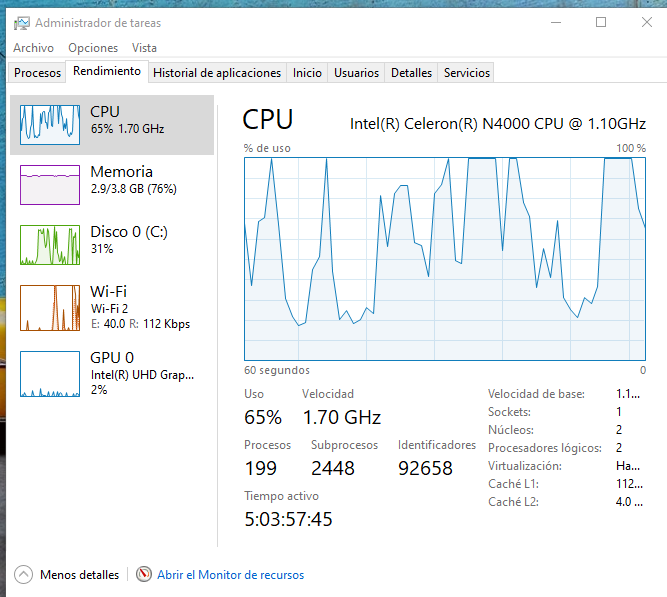
\includegraphics[width=10cm]{CPU.png}
 \caption{Nucleos del procesador.}
 \label{f1}
\end{center}
\end{figure}


\section{Resultados y Discusi\'{o}n.}\label{res}

Una vez obtenido el c\'odigo\citep{ana} se realizaron algunas variaciones entre el tiempo original el invertido y el aleatorio, as\'i mismo se corrio el c\'odigo varias veces para diferentes magnitudes del vector, tomando n\'umeros de entre 1,10,100,1000,3000 de diferencia de un n\'umero primo a otro.

\begin{figure}[h!]
       \centering
       \begin{subfigure}[b]{0.45\linewidth}
           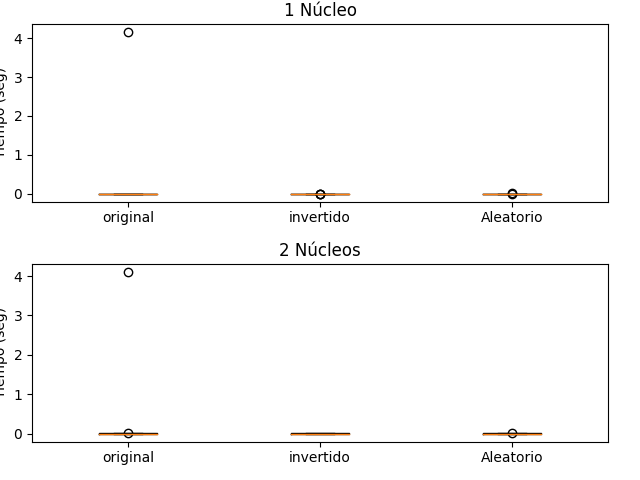
\includegraphics[width=\linewidth]{Figure_1.png}
           \caption{Variaci\'on 1}
           \label{fig:westminster_lateral}
        \end{subfigure}
        \begin{subfigure}[b]{0.45\linewidth}
            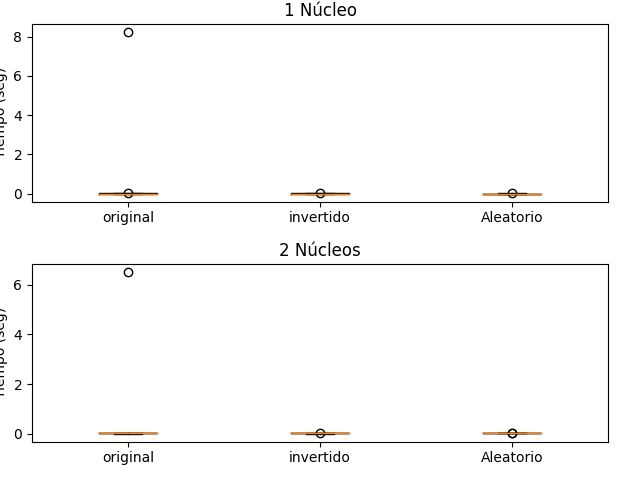
\includegraphics[width=\linewidth]{Figure_1(10).png}
            \caption{Variaci\'on 10}
            \label{fig:westminster_aerea}
        \end{subfigure}
        \begin{subfigure}[b]{0.45\linewidth}
           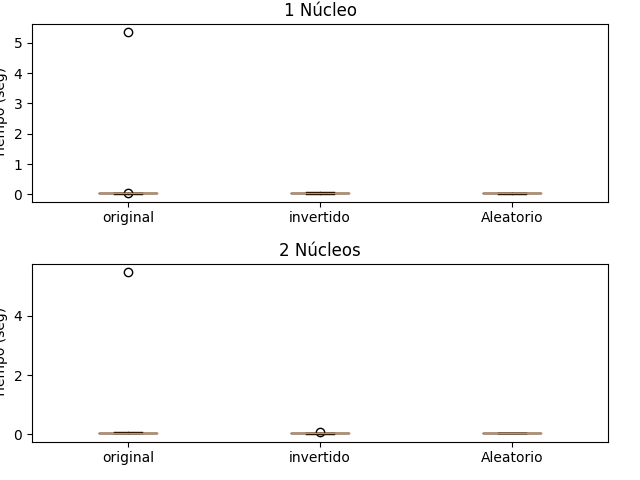
\includegraphics[width=\linewidth]{Figure_1(100).png}
           \caption{Variacion 100}
           \label{fig:westminster_aerea}
        \end{subfigure}
        \begin{subfigure}[b]{0.45\linewidth}
           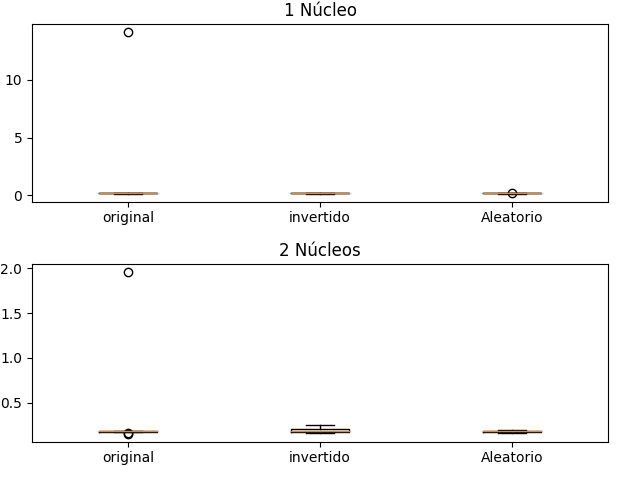
\includegraphics[width=\linewidth]{Figure_1(1000).png}
           \caption{Variaci\'on 1000}
           \label{fig:westminster_aerea}
        \end{subfigure}
      \begin{subfigure}[b]{0.45\linewidth}
           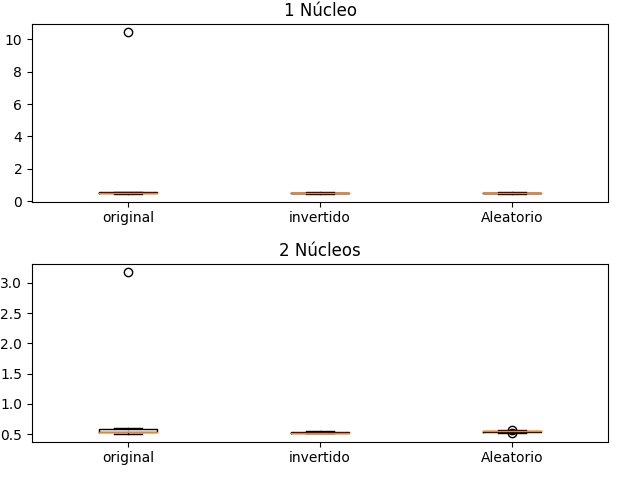
\includegraphics[width=\linewidth]{Figure_1(3000).png}
           \caption{Variaci\'on 3000}
           \label{fig:westminster_aerea}
        \end{subfigure}
        \caption{Magnitudes del vector}
        \label{fig:westminster}
\end{figure}

As\'i mismo tomando en cuenta la variaci\'on de nucleos se observan los resultados en los tiempos contra nucleos.

\begin{figure}[h!]
       \centering
       \begin{subfigure}[b]{0.45\linewidth}
           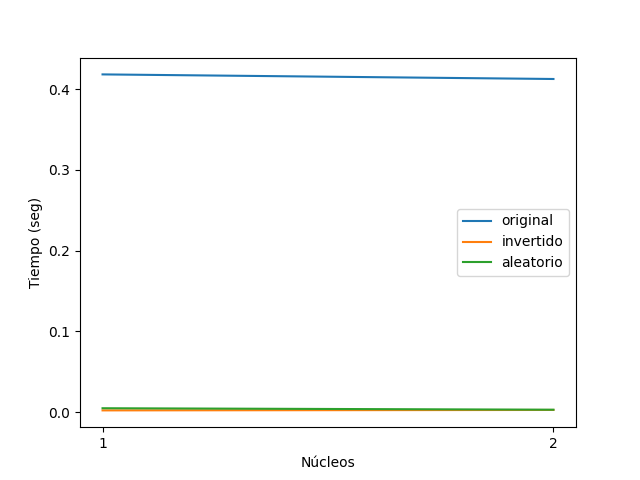
\includegraphics[width=\linewidth]{Figure_1.1.png}
           \caption{Variaci\'on 1}
           \label{fig:westminster_lateral}
        \end{subfigure}
        \begin{subfigure}[b]{0.45\linewidth}
            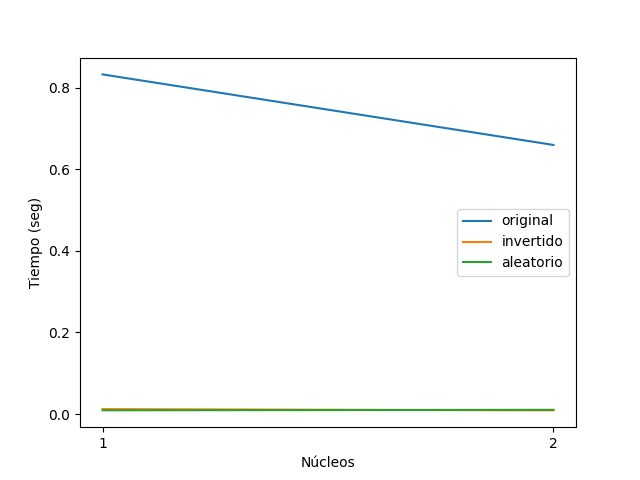
\includegraphics[width=\linewidth]{Figure_1.1(10).png}
            \caption{Variaci\'on 10}
            \label{fig:westminster_aerea}
        \end{subfigure}
        \begin{subfigure}[b]{0.45\linewidth}
           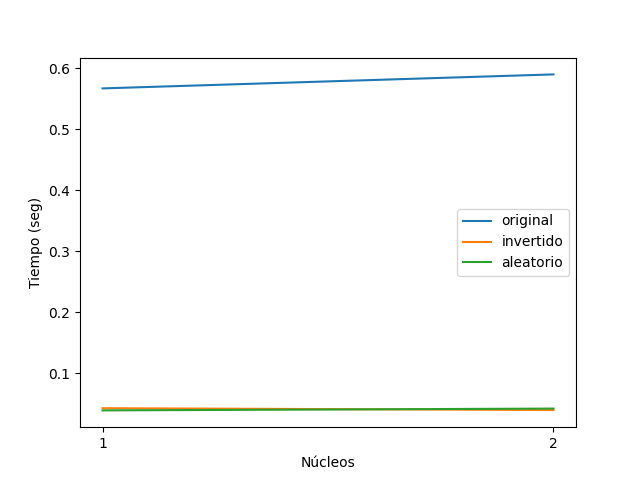
\includegraphics[width=\linewidth]{Figure_1.(100).png}
           \caption{Variaci\'on 100}
           \label{fig:westminster_aerea}
        \end{subfigure}
        \begin{subfigure}[b]{0.45\linewidth}
           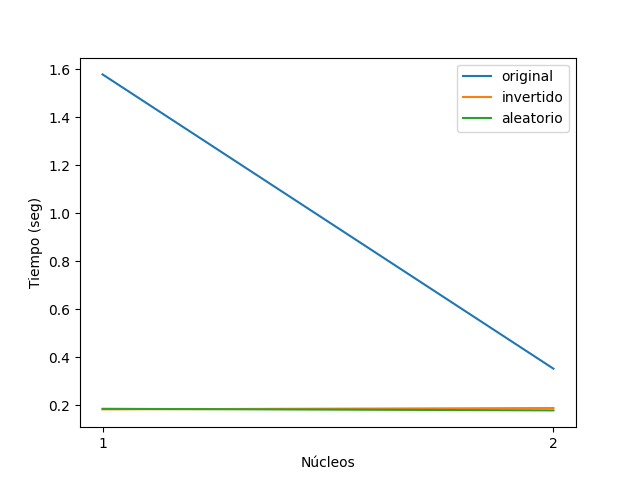
\includegraphics[width=\linewidth]{Figure_1.1(1000).png}
           \caption{Variaci\'on 1000}
           \label{fig:westminster_aerea}
        \end{subfigure}
      \begin{subfigure}[b]{0.45\linewidth}
           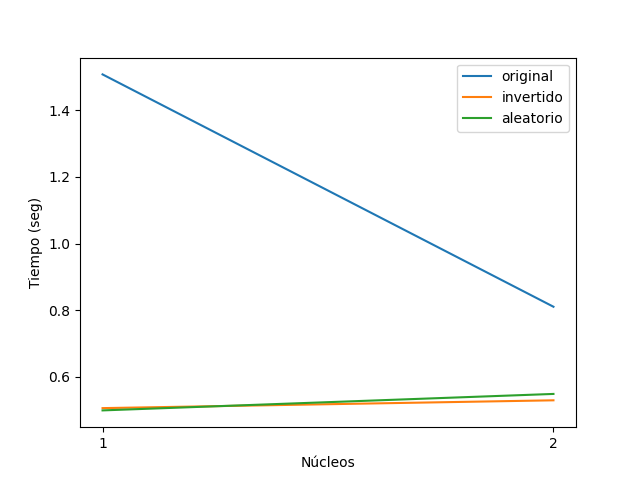
\includegraphics[width=\linewidth]{Figure_1.1(3000).png}
           \caption{Variaci\'on 3000}
           \label{fig:westminster_aerea}
        \end{subfigure}
        \caption{Tiempo Vs N\'ucleos}
        \label{fig:westminster}
\end{figure}

De igual manera los datos estadisticos como el m\'aximo,el m\'inimo etc, se encuentran en la tabla \ref{t1}.

\begin{table} 
 \caption{datos esta\'isticos de los tiempos de ejecuci\'on.}
 \label{t1}
 \begin{center}
 \begin{tabular}{rrrrrrr}
\texttt{Ordenamiento} & \texttt{Min} & \texttt{Max} &\texttt{Mean} & \texttt{Variace}  & \texttt{Skewness} & \texttt{Kurtosis} \\
Original (1  n\'ucleos) & 0.47 &10.45  & 1.50 & 9.8819 & 2.66 & 5.10 \\ 
Invertido (1  n\'ucleos) & 0.46 & 0.56 & 0.50 & 0.001 & 0.26 & -1.12\\ 
Aleatorio(1 n\'ucleos) & 0.46& 0.56 & 0.49 & 0.001 & 0.756 & -0.429 \\ 
Original (2 n\'ucleos) &0.5105  &3.177  & 0.810 &0.692  &2.661 &5.094  \\ 
Invertido (2 n\'ucleos) & 0.5157 &0.557 & 0.529 &  0.00021&0.680 & -0.813 \\ 
Aleatorio (2 n\'ucleos) & 0.5238 &0.576  & 0.549 &0.00027  & -0.051 & -0.674 \\ 
\end{tabular}
\end{center}
\end{table}

  \section{Conclusi\'{o}n.}\label{con}
El n\'umero de n\'ucleos que se asigna para la ejecuci\'on tiene un impacto muy grande en el tiempo que le toma realizar el an\'alisis, sin embargo no se pudo observar con m\'as de dos n\'ucleos, de igual forma el n\'umero de datos entre primos y no primos que se an\'alizan es un factor imprtante en cuanto al tiempo que le tome analizarlos, mientras mayor sea la magnitud del vector mayor sera el tiempo que le tome an\'alizar.
  \bibliography{consulta}
  \bibliographystyle{plainnat}
\end{document}